%% by Michael Shell
%% Edited by Rodrigo Almeida
%%
%% This work is distributed under the LaTeX Project Public License (LPPL)
%% ( http://www.latex-project.org/ ) version 1.3, and may be freely used,
%% distributed and modified. A copy of the LPPL, version 1.3, is included
%% in the base LaTeX documentation of all distributions of LaTeX released
%% 2003/12/01 or later.
%% Retain all contribution notices and credits.

\documentclass[10pt,journal,compsoc]{IEEEtran}

\hyphenation{op-tical net-works semi-conduc-tor}

\usepackage{hyperref}
\usepackage{biblatex}
\usepackage{graphicx}
\usepackage{listings}
\usepackage{multirow}
\usepackage{tabularx}
\usepackage{caption}
\usepackage{booktabs}
\usepackage{listings}
\usepackage{xcolor}
\usepackage{float}
\lstset{
    basicstyle=\ttfamily\footnotesize,
    keywordstyle=\color{blue},
    commentstyle=\color{green!30!black},
    stringstyle=\color{red},
    showstringspaces=false,
    breaklines=true,
    frame=single,
}

\graphicspath{{images/}}

\addbibresource{references.bib}

\begin{document}
% paper title
% Titles are generally capitalized except for words such as a, an, and, as,
% at, but, by, for, in, nor, of, on, or, the, to and up, which are usually
% not capitalized unless they are the first or last word of the title.
% Linebreaks \\ can be used within to get better formatting as desired.
% Do not put math or special symbols in the title.
% \title{Transparency in AI - Decision-Making with Explainable AI (XAI)}
\title{Why Explain a decision made by AI? Explainable AI (XAI)}

% author name
\author{Rodrigo Almeida% <-this % stops a space
}

% The paper headers
\markboth{Research Methods in Computing \& IT - Literature Review}%
{}

\IEEEtitleabstractindextext{
    \begin{abstract}
        In this paper, I will review the literature relating to transparency for decisions made by artificial intelligence (AI). As AI advances, not only our dependence on AI models are increasing but also a need for understanding how such results and decisions were made by the model. Due to the complexity of AI, Explainable Artificial Intelligence (XAI) has become a great choice, bringing more clarity, where outputs can be explained reducing bias and bringing transparency to the decision-making process, as opposed to "Black Box" algorithms that we cannot explain why or how the AI arrived in such a conclusion/classification/decision, it outputs directly from data, and not even who developed such algorithms are able to explain how the model arrived in such result.


    \end{abstract}
}

% make the title area
\maketitle

\section{Introduction}
\label{sec:introduction}

\IEEEPARstart{E}xplainable AI is emerging, and with it, the concerns from scientists, the general public and policymakers are also on the rise. As artificial intelligence, machine learning and deep learning are becoming integrated into applications, decisions from such models can carry consequences for a person and society, changing the focus from accuracy to the necessity of being able to explain and clarify how these decisions were made.\cite{analytical-review} As we are becoming more dependent and relying hugely on intelligent machines, whether it is email filters, AI helping with medical diagnoses or self-driving cars, machine learning is being used across almost all sectors. Such growth in these technologies only highlights the importance of understanding the interpretability of the outcome generated by it. This is the main motivation for explainable artificial intelligence.\cite{doshivelez2017rigorous}
The impact of the outcome will vary based on the field. A wrong prediction for computing and business might lead to misleading recommendations, potentially affecting the revenue of such businesses, however wrong predictions in critical sectors like healthcare could put human life at risk. Opening the "black box" is incredibly important, not just for social acceptance but also for regulatory purposes. Understanding how AI systems reach their conclusions is crucial in ensuring accountability, transparency, and ethical use of these technologies, making it essential for both public trust and regulatory compliance.\cite{analytical-review}

In \autoref{fig:xaiGraphic} we can easily understand the main differences between the "Black Box" and XAI.\cite{xai-concept}

\begin{figure}[h]
    \centering
    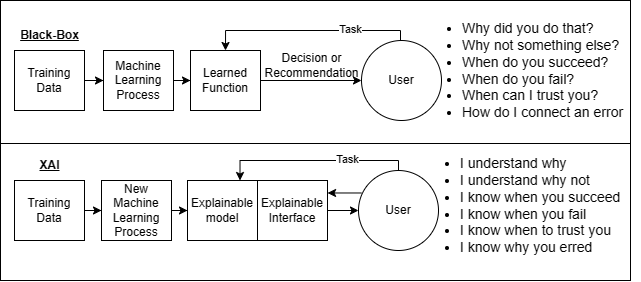
\includegraphics[scale=0.37]{images/xaiGraphic.png}
    \caption{XAI Concept}
    \label{fig:xaiGraphic}
\end{figure}

\section{Definitions}

Explainable AI (XAI) is a field focused on increasing human understanding of AI systems. Although terms like transparency, interpretability, and explainability are frequently used together, they can have different meanings, there are differences between these theories.\cite{xai-ml}

\begin{itemize}
    \item {Transparency}: a model deemed transparent is one that can be understood easily on its own. It is the opposite of a "black box", indicating that the inner workings of the model are understandable\cite{transparency}.
    \item {Interpretability}: It is the ability to explain concepts that are complex or result in a way that humans will easily understand\cite{gilpin2019explaining}.
    \item {Explainability}: it is the concept that provides explanations as a bridge between AI systems and humans. It involves the ability to create AI systems that are not only accurate but also people can understand.\cite{gilpin2019explaining}.
\end{itemize}

\section{Overview of Explainable AI Algorithms}
Researchers have developed many algorithms to explain AI systems. These explanations could be categorized into two primary groups: self-interpretable models refer to the algorithm model itself or a representation of the algorithm that can be directly read and comprehended by a human. In this case, the model itself serves as the explanation. On the other hand, post-hoc explanations are descriptions, explanations, or models of the algorithm often produced by separate software tools. These tools aim to provide an understanding of how the algorithm operates. Post-hoc explanations are particularly useful for algorithms for which the inner workings are not fully transparent, as they can be employed to generate insights without requiring deep knowledge of the algorithm's internal mechanisms. Instead, they rely on querying the algorithm for outputs based on selected inputs.\cite{phillips2020four}.

\subsection{Self-interpratable Models}
Models that are self interpratable are those that serve as the explanation themselves. They not only describe the entire model but also it goes through each input, replicating the input on the self-interpretable model can providing a justification for each decision.
Common self-interpretable models are decision trees and regression models. Ongoing research aims to create more interpretable models that surpass the accuracy of basic decision trees and regression models. These newer models include decision lists, decision sets, prototypes (representative samples of each class), feature combination rules, Bayesian Rule Lists, additive decision trees, and improved versions of decision trees.\cite{phillips2020four}
Some sources suggest there is a trade-off between accuracy and interpretability with self-interpretable models being less accurate than post-hoc models. The challenge, in this case, is really to balance the precision of the model with what it means to humans. However, scholars like Rudin\cite{rudin} and Radin\cite{radin} in their research called "Why Are We Using Black Box Models in AI When We Don’t Need To? A Lesson From an Explainable AI Competition", disagree, explaining that there is not necessarily a trade-off between accuracy and interpretability. In many cases, interpretable models can be utilized without sacrificing decision accuracy.\cite{phillips2020four}

\subsection{Pos-hoc Explanations}
Post-hoc explanations refer to an explanation given after a model has been trained. In other words, the explanations are generated after the model has made the decision or prediction and not during the training phase. It is divided into two: local explanation and global explanation.

\subsection{Local Explanation} Local explanations explain a subset of inputs. It focuses on explaining the output for a specific data point. The most common type is a per-decision or single-decision explanation, which gives an explanation for the output or decision on a single input.\cite{phillips2020four}
These explanations focus on a single prediction and aim to answer the following question: "Why did this model make that particular prediction for that specific task?" There are some techniques used for local explanation. Some of the techniques used for local explanation are:

\subsubsection{LIME - Local Interpretable Model-agnostic Explainer}
LIME takes a specific decision made by an ML model, and examines nearby data points, creating a simplified and interpretable model that represents a decision made locally\cite{phillips2020four}. The default model is logistic regression.
When dealing with images, LIME breaks down the image into smaller regions called superpixels. It then explores combinations of these superpixels omitting some and replacing some with black. By doing this, LIME aims to understand and explain how the model's decision is influenced by specific parts of the image.

\subsubsection{SHAP - SHapley Additive exPlanations} SHAP is based on concepts of game theory and can explain the predictions by calculating the contribution of every feature to the prediction. It provides an understanding of how each feature impacts every model's prediction by considering their interaction in a consistent and fair way. This helps increase the interpretability by explaining the logic behind every prediction.\cite{why-trust-you}

\subsection{Global Explanations}
Global explanations produce post-hoc explanations throughout the whole dataset. It outlines the process used for the decision-making, mentioning tendencies,\\
features and possible biases that the model should have learned from the data. Global explanations are essential to understanding the model's behaviours and,  ensuring fairness, identifying biases, and increasing trust in AI systems. \\
Such context in XAI helps stakeholders to cope with potential issues understanding the impact and implications of decisions made by a model. Some of the techniques used for global explanation are:

\subsubsection{PDPs - Partial Dependence Plots}
PDPs show the change in the response when a value changes in the feature, showing some insights about the relationship between the feature and the response. It is particularly useful when trying to determine if the relationship between a feature and the response is linear or more complex, understanding how the model behaves for individual features.\cite{phillips2020four}

\subsubsection{ICE - Individual Conditional Expectation Curves}
Individual conditional expectation curves are a more user-friendly way to understand how a feature influences a prediction for a single instance. by doing so, it makes it easier to understand how the model behaves for a specific case.

\subsubsection{TCAV - Testing with Concept Activation Vectors}
This is a global algorithm designed to explain neural networks in a way that is easier to understand. It represents the neural network state using a linear interpretation of the internals of deep learning.

\subsubsection{CAVs - Concept Activation Vectors}
Concept Activation Vectors are user-friendly concepts used by TCAV to explain neural networks. It is the numerical representation of a concept, making it more understandable to humans.

\subsubsection{Decision sets}
Opposite to black-box models, the decision sets capture the decision-making process by generating a set of rules outlining the conditions in which the model predicts certain outcomes, helping understand the model's decision boundaries.

\subsubsection{LIME }
The Local Interpretable model-agnostic explanations aim to approximate any black-box machine learning model with a local and interpretable model explaining each individual prediction.

\section{Interpreting Predictions - A Case Study with the "Adult Income" dataset}
As a case study, I will use the "Adult Income" data set\cite{misc_adult_2} to predict whether an individual earns more than €50,000/year based on 14 features. This dataset was extracted by Barry Becker and is often cited in machine learning literature and research papers.
Table \ref{tab:variable-descriptions} shows the 14 features listed by name, role type and demographic.

\begin{table}[h]
    \centering
    \small
    \begin{tabularx}{\columnwidth}{|p{1.8cm}|X|X|}
        \hline
        \textbf{Aspect}           & \textbf{Local Explanation}                                                                                              & \textbf{Global Explanation}                                                                                                                                    \\
        \hline
        \textbf{Scope}            & It explains individual predictions.                                                                                     & It will focus on understanding the model's behaviour across the entire dataset.                                                                                \\
        \hline
        \textbf{Granularity}      & Aims to explain why a particular decision was made.                                                                     & Higher level overview of the model's behaviour, bringing up general trends and feature importance across the dataset.                                          \\
        \hline
        \textbf{Techniques}       & LIME, SHAP, individual instance inspection.                                                                             & PDPs, ICE, SP-LIME, TCAV, decision sets, summary of counterfactual rules.\cite{phillips2020four}                                                               \\
        \hline
        \textbf{Use Cases}        & Focus on explaining why a specific prediction was made, especially in critical applications like healthcare or finance. & Focus on identifying biases, ensuring fairness, and gaining an overall understanding of the model's behaviour for regulatory compliance and model improvement. \\
        \hline
        \textbf{Interpretability} & Easier to understand for individual cases, focusing on the explanation specific.                                        & Wider view of the model, making it valuable for stakeholders and policymakers seeking a general understanding of the AI system.                                \\
        \hline
    \end{tabularx}
    \caption{Comparison of Local and Global Explanations in XAI}
    \label{tab:xai_comparison}
\end{table}

\section{Interpreting Predictions - A Case Study with the "Adult Income" dataset}
As a case study, I will use the "Adult Income" data set\cite{misc_adult_2} to predict whether an individual earns more than €50,000/year based on 14 features. This dataset was extracted by Barry Becker and is often cited in machine learning literature and research papers.
Table \ref{tab:variable-descriptions} shows the 14 features listed by name, role type and demographic.

\begin{table}[h]
    \centering
    \caption{Variable Descriptions}
    \begin{tabularx}{\columnwidth}{cccccc}
        \toprule
        \textbf{Variable Name} & \textbf{Role} & \textbf{Type} & \textbf{Demographic} \\
        \midrule
        age                    & Feature       & Integer       & Age                  \\
        workclass              & Feature       & Categorical   & Income               \\
        fnlwgt                 & Feature       & Integer       & ---                  \\
        education              & Feature       & Categorical   & Education Level      \\
        education-num          & Feature       & Integer       & Education Level      \\
        marital-status         & Feature       & Categorical   & Other                \\
        occupation             & Feature       & Categorical   & Other                \\
        relationship           & Feature       & Categorical   & Other                \\
        race                   & Feature       & Categorical   & Race                 \\
        sex                    & Feature       & Binary        & Sex                  \\
        capital-gain           & Feature       & Integer       & ---                  \\
        capital-loss           & Feature       & Integer       & ---                  \\
        hours-per-week         & Feature       & Integer       & ---                  \\
        native-country         & Feature       & Categorical   & Other                \\
        income                 & Target        & Binary        & Income               \\
        \bottomrule
    \end{tabularx}
    \label{tab:variable-descriptions}
\end{table}

\begin{itemize}
    \item \textbf{Age:} It represents the age of a person, it is an important factor in predicting income because the age can reflect an individual's level of experience and earning potential.

    \item \textbf{Workclass:} It can be categorized in Private, Self-emp-not-inc, Self-emp-inc, Federal-gov, Local-gov, State-gov, Without-pay, Never-worked. It refers to the type of employment. Status of employment is also an important factor, as income levels often vary according to employment status.

    \item \textbf{Fnlwgt:} Final weight represents the number of people the census believes the entry represents.

    \item \textbf{Education Level:} Represents the highest level of education an individual has obtained. It is divided into Bachelors, Some-college, 11th, HS-grad, Prof-school, Assoc-acdm, Assoc-voc, 9th, 7th-8th, 12th, Masters, 1st-4th, 10th, Doctorate, 5th-6th, Preschool. The education level is a key predictor of income since individuals with higher education often have access to better-paying job opportunities.

    \item \textbf{Education Num:} This is a numerical representation of the educational level. This also helps understand the education obtained by an individual.

    \item \textbf{Marital Status:} This describes the marital status of the individual. It is divided into Married-civ-spouse, Divorced, Never-married, Separated, Widowed, Married-spouse-absent, and Married-AF-spouse.

    \item \textbf{Occupation:} Specifies the type of education the individual is involved with. It is divided into Tech-support, Craft-repair, Other-service, Sales, Exec-managerial, Prof-specialty, Handlers-cleaners, Machine-op-inspct, Adm-clerical, Farming-fishing, Transport-moving, Priv-house-serv, Protective-serv, Armed-Forces. Occupation is also a key factor which influences income, as the income levels are different depending on the occupation.

    \item \textbf{Relationship:} This describes the relationship status of an individual which can have an impact on household income and financial stability. It is divided into Wife, Own-child, Husband, Not-in-family, Other-relative, and Unmarried.

    \item \textbf{Race:} Indicates the race of the individual. It shouldn't directly affect income but could be linked to other socioeconomic factors that can impact earnings. It is divided into White, Asian-Pac-Islander, Amer-Indian-Eskimo, Other, and Black.

    \item \textbf{Sex:} Specifies the gender of the individual. It can influence income for reasons such as wage gaps and job segregation. It is divided into Female and Male.

    \item \textbf{Capital Gain:} Represents capital gains for the individual. It contributes to overall income.

    \item \textbf{Capital Loss:} Represents capital losses for the individual. It can impact the individual's financial situation.

    \item \textbf{Hours Per Week:} Indicates the number of working hours per week. The number of hours worked in a week influences the income directly.

    \item \textbf{Native Country:} Indicates the individual's country of origin. Depending on the country of origin the individual may be impacted by less or more opportunities. It is divided into: United-States, Cambodia, England, Puerto-Rico, Canada, Germany, Outlying-US(Guam-USVI-etc), India, Japan, Greece, South, China, Cuba, Iran, Honduras, Philippines, Italy, Poland, Jamaica, Vietnam, Mexico, Portugal, Ireland, France, Dominican-Republic, Laos, Ecuador, Taiwan, Haiti, Columbia, Hungary, Guatemala, Nicaragua, Scotland, Thailand, Yugoslavia, El-Salvador, Trinadad \& Tobago, Peru, Hong, Holand-Netherlands.

    \item \textbf{Income:} This is the target variable indicating whether the individual's income exceeds  \$50,000 per year. This is the variable we are trying to predict.

\end{itemize}

\subsection{Using Python to interpret predictions}
In this section, I will use Python to interpret predictions made by a machine learning model, using the "Adult Income" described above.

\subsubsection{Importing the libraries}

\begin{lstlisting}[language=Python, caption={Import libraries}, label=python_code, captionpos=b,  basicstyle=\scriptsize]
    # Import necessary libraries
    import pandas as pd
    from sklearn.model_selection import train_test_split
    from sklearn.tree import DecisionTreeClassifier, plot_tree
    from sklearn.ensemble import RandomForestClassifier
    from sklearn.metrics import accuracy_score
    import shap
    from lime import lime_tabular
    import matplotlib.pyplot as plt
\end{lstlisting}

\subsubsection{Loading the dataset}
\begin{lstlisting}[language=Python, caption={Load dataset}, label=python_code, captionpos=b,  basicstyle=\scriptsize]
    # Load the Adult Income dataset (replace 'path_to_data' with your actual path)
    data_url = "https://archive.ics.uci.edu/ml/machine-learning-databases/adult/adult.data"
    columns = ['age', 'workclass', 'fnlwgt', 'education', 'education-num', 'marital-status', 'occupation',
               'relationship', 'race', 'sex', 'capital-gain', 'capital-loss', 'hours-per-week', 'native-country', 'income']
    data = pd.read_csv(data_url, header=None, names=columns, na_values=' ?', skipinitialspace=True)
    data.describe()
    data
  
    
\end{lstlisting}

\subsubsection{Data Preprocessing}

\begin{lstlisting}[language=Python, caption={Data Preprocessing}, label=python_code, captionpos=b,  basicstyle=\scriptsize]
    # Preprocess the data
    data = data.dropna()
    data_encoded = pd.get_dummies(data, columns=['workclass', 'education', 'marital-status', 'occupation', 'relationship', 'race', 'sex', 'native-country'])
    X = data_encoded.drop('income', axis=1)
    y = data_encoded['income']
\end{lstlisting}

\subsubsection{Splitting the dataset into training and test sets}
\begin{lstlisting}[language=Python, caption={Splitting the dataset into training and test sets}, label=python_code, captionpos=b,  basicstyle=\scriptsize]
    # Split the data into training and testing sets
    X_train, X_test, y_train, y_test = train_test_split(X, y, test_size=0.2, random_state=42)
  
\end{lstlisting}

\subsubsection{Training a Decision Tree Classifier}

\begin{lstlisting}[language=Python, caption={Training a Decision Tree Classifier}, label=python_code, captionpos=b,  basicstyle=\scriptsize]
    # Train a decision tree model
    decision_tree_model = DecisionTreeClassifier(random_state=42)
    decision_tree_model.fit(X_train, y_train)
    
    # Evaluate the Decision Tree model
    y_pred_dt = decision_tree_model.predict(X_test)
    accuracy_dt = accuracy_score(y_test, y_pred_dt)
    print(f"Decision Tree Accuracy: {accuracy_dt}")
    
\end{lstlisting}

\subsubsection{Simplify feature names for visualization}
\begin{lstlisting}[language=Python, captionpos=b,  basicstyle=\scriptsize]
    # Simplify feature names for visualization
    feature_names_simplified = [col.split('_')[0] if '_' in col else col for col in X.columns]
\end{lstlisting}

\textbf{Decision Tree Accuracy: 0.82081989866421}


\subsubsection{Visualize the Decision Tree}
\begin{lstlisting}[language=Python, caption={Visualize the Decision Tree}, label=python_code, captionpos=b,  basicstyle=\scriptsize]
    # Feature importances from the Decision Tree
    feature_importances = decision_tree_model.feature_importances_
    # Create a bar plot for feature importances
    plt.figure(figsize=(12, 8))
    plt.barh(feature_names_simplified, feature_importances)
    plt.xlabel('Feature Importance')
    plt.title('Decision Tree Feature Importances')
    plt.show()    
\end{lstlisting}

\begin{figure}[H]
    \centering
    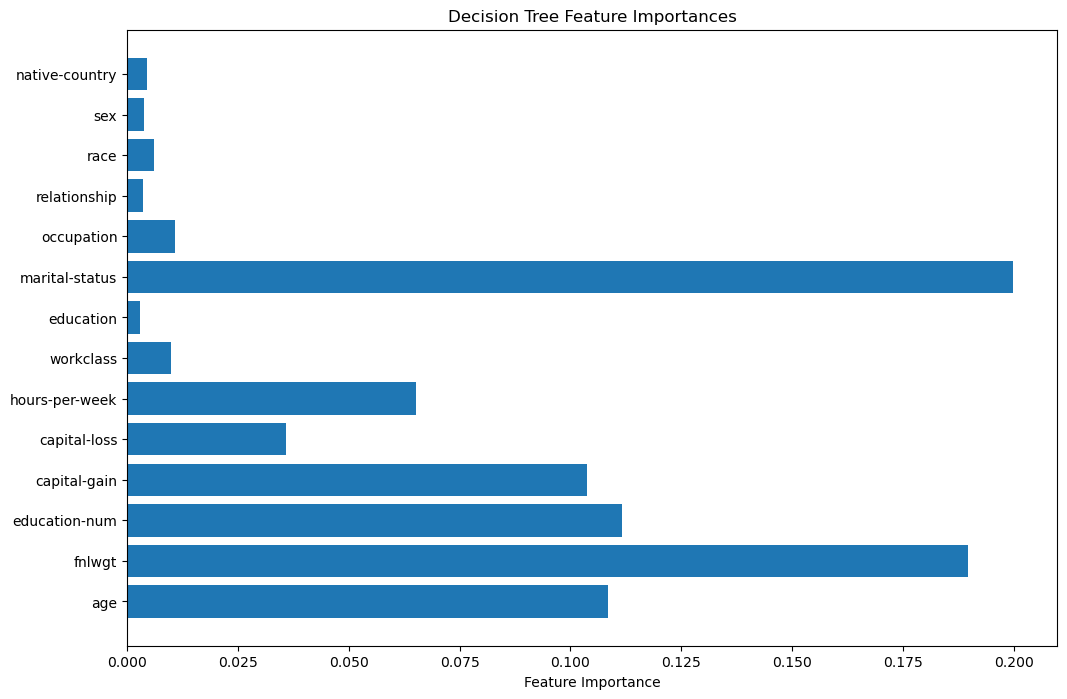
\includegraphics[width=1\linewidth]{images/decision_tree_feature_importances.png}
    \caption{Decision Tree Feature Importances}
    \label{fig:decision_tree_feature_importances}
\end{figure}

\subsubsection{Apply SHAP for Global Explanations}

\begin{lstlisting}[language=Python, caption={Apply Post-Hoc Explanations}, label=python_code, captionpos=b,  basicstyle=\scriptsize]
    # Apply SHAP for global explanations
    shap_values_dt = shap.TreeExplainer(decision_tree_model).shap_values(X)
    
    # Generate bar charts for SHAP values
    shap.summary_plot(shap_values_dt[1], X, feature_names=feature_names_simplified, class_names=['<=50K', '>50K'], plot_type='bar')
    
\end{lstlisting}

\begin{figure}[h]
    \centering
    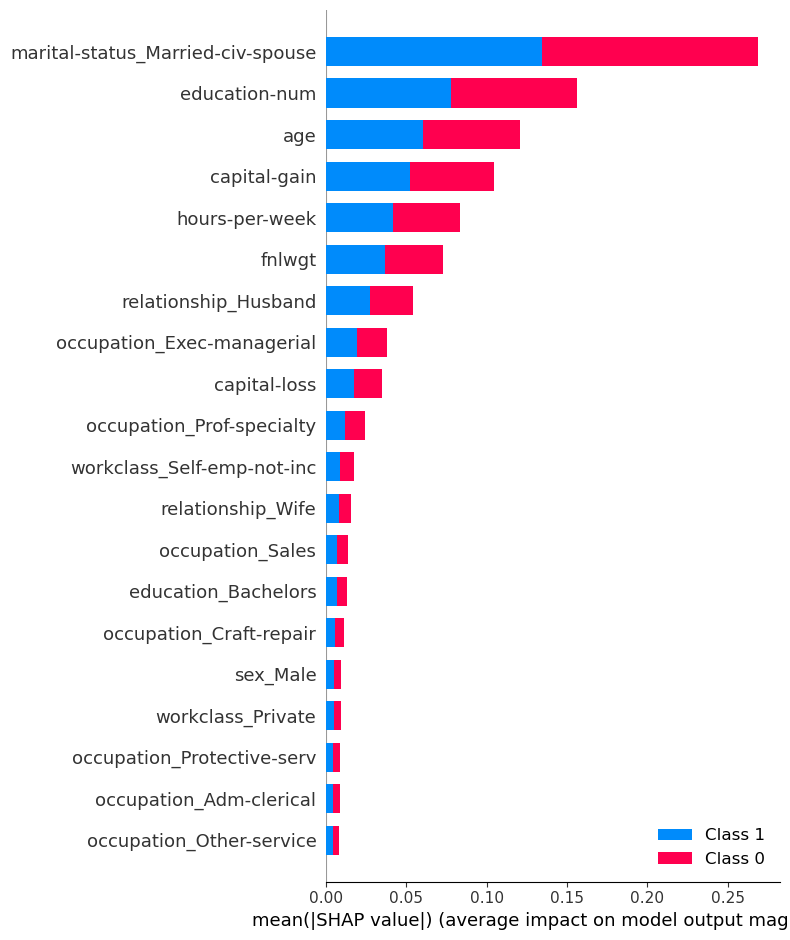
\includegraphics[width=0.9\linewidth]{images/shap_summary_plot.png}
    \caption{SHAP Summary Plot}
    \label{fig:shap_summary_plot}
    \end{figure}


\section{Future Work}


\section{Conclusion}



% references section
\printbibliography

\end{document}